\chapter{Results}\label{CH5}
Present the results from following the procedures in \nameref{CH4}, note some observations, but do not discuss them.

\begin{table}[h]
    \centering
    \begin{tabular}{l | l | l}
    A & B & C \\
    \hline
    1 & 2 & 3 \\
    4 & 5 & 6
    \end{tabular}
    \caption{very basic table}
    \label{tab:abc}
    \end{table}

\begin{figure}
    \centering
    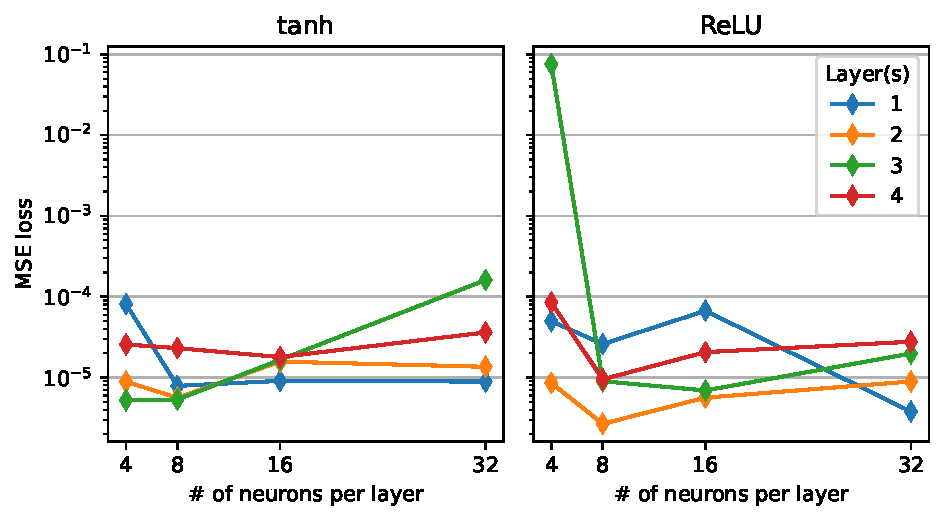
\includegraphics[width=\textwidth]{results/para1_net}
    \caption{Final training losses for different network architectures defined by activation function, number of hidden layers and number of neurons per hidden layer}
    \label{fig:para1_net}
\end{figure}

\begin{figure}
    \centering
    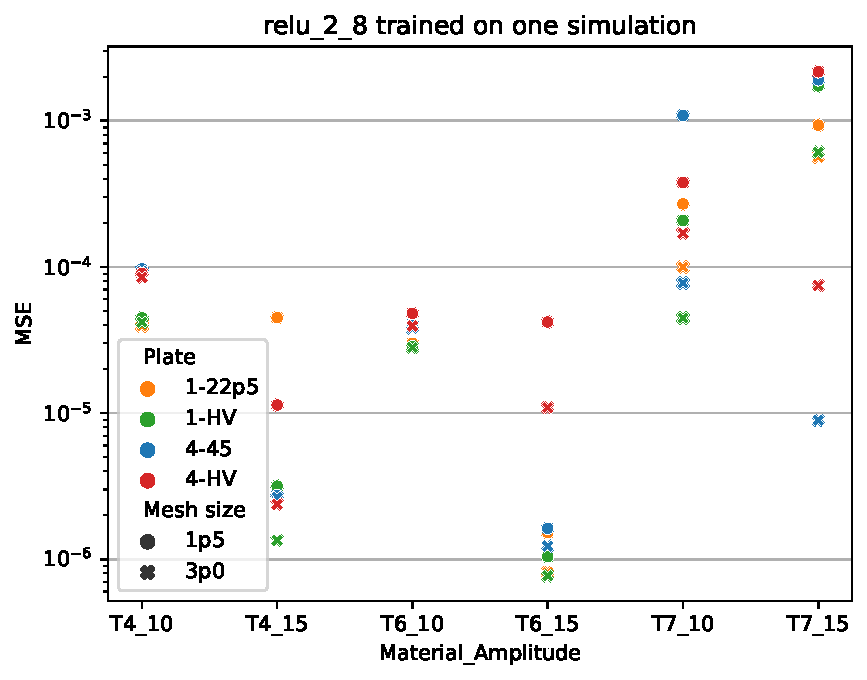
\includegraphics[width=\textwidth]{results/para1_all}
    \caption{Bottom text}
    \label{fig:para1_all}
\end{figure}

\begin{figure}
    \centering
    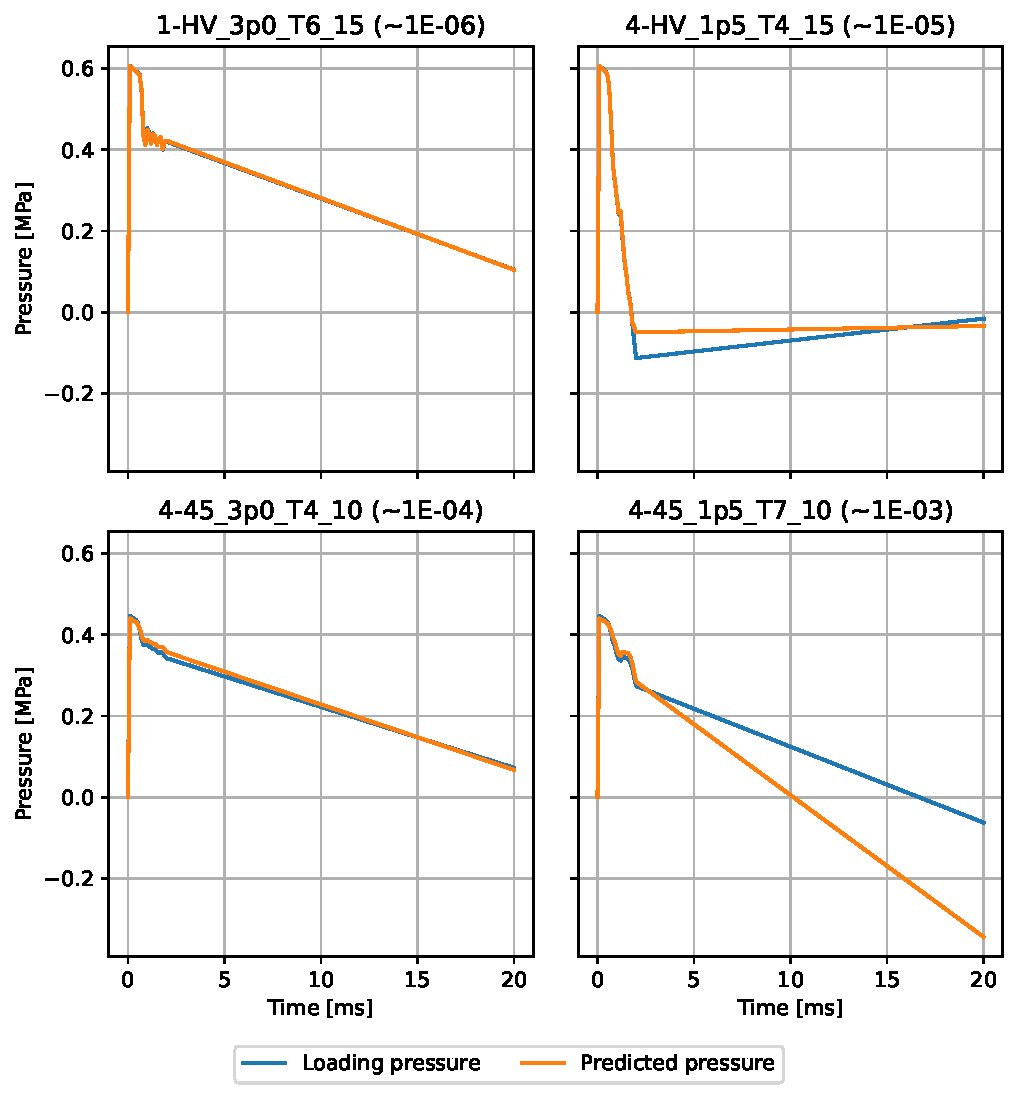
\includegraphics[width=\textwidth]{results/para1_test}
    \caption{Bottom text}
    \label{fig:para1_test}
\end{figure}

\begin{figure}
    \centering
    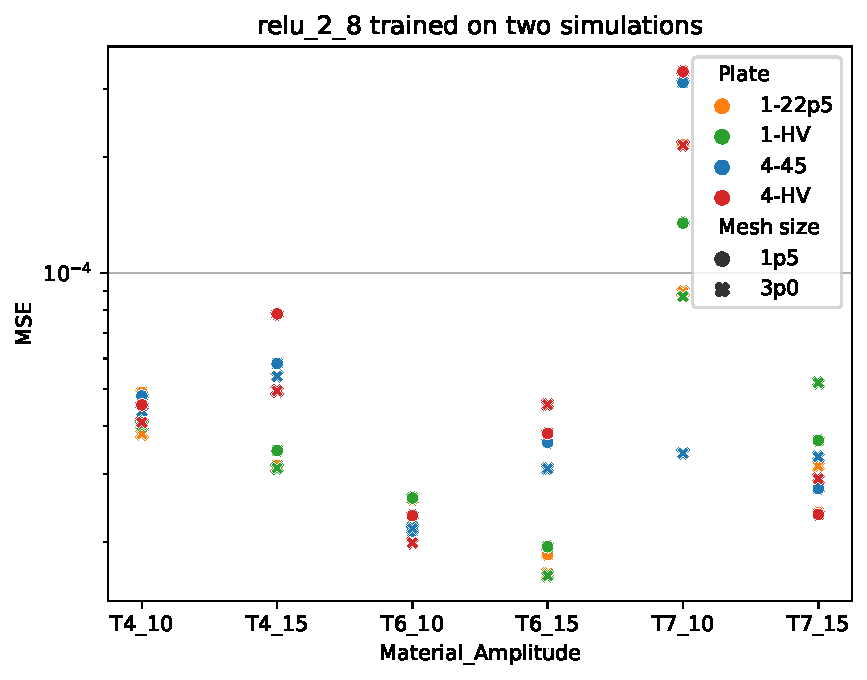
\includegraphics[width=\textwidth]{results/para2_all}
    \caption{Bottom text}
    \label{fig:para2_all}
\end{figure}

\begin{figure}
    \centering
    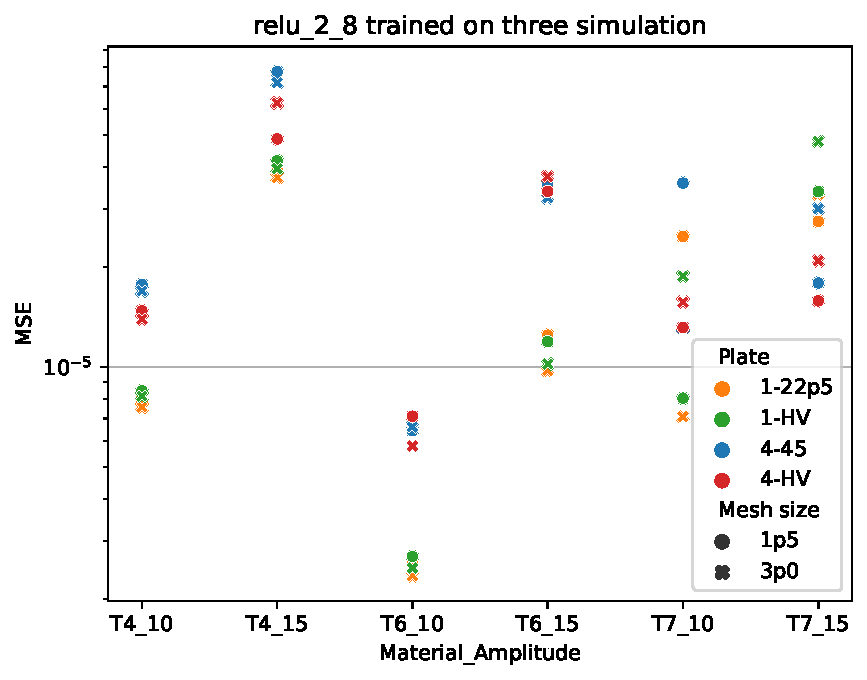
\includegraphics[width=\textwidth]{results/para3_all}
    \caption{Bottom text}
    \label{fig:para3_all}
\end{figure}

\begin{figure}
    \centering
    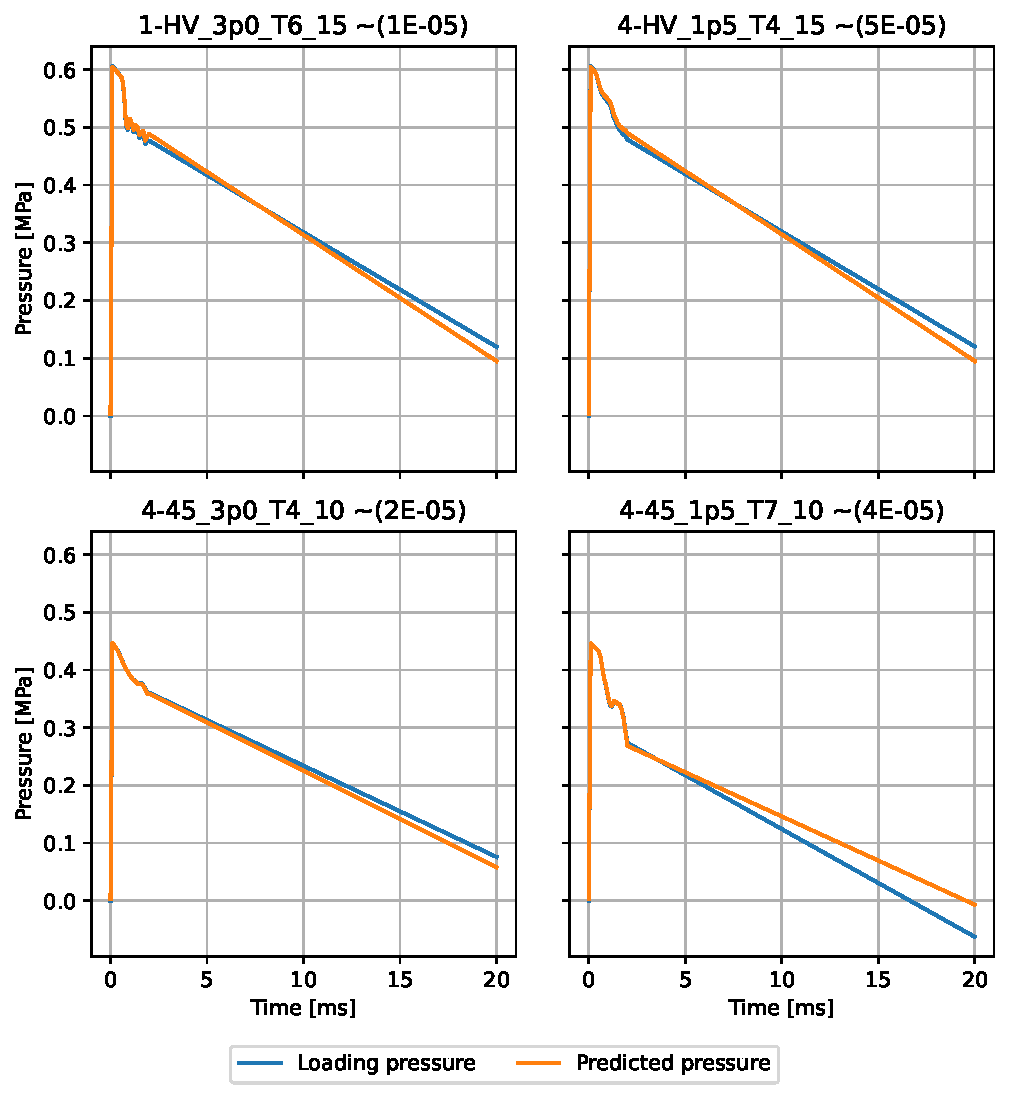
\includegraphics[width=\textwidth]{results/para3_test}
    \caption{Bottom text}
    \label{fig:para3_test}
\end{figure}

\begin{figure}
    \centering
    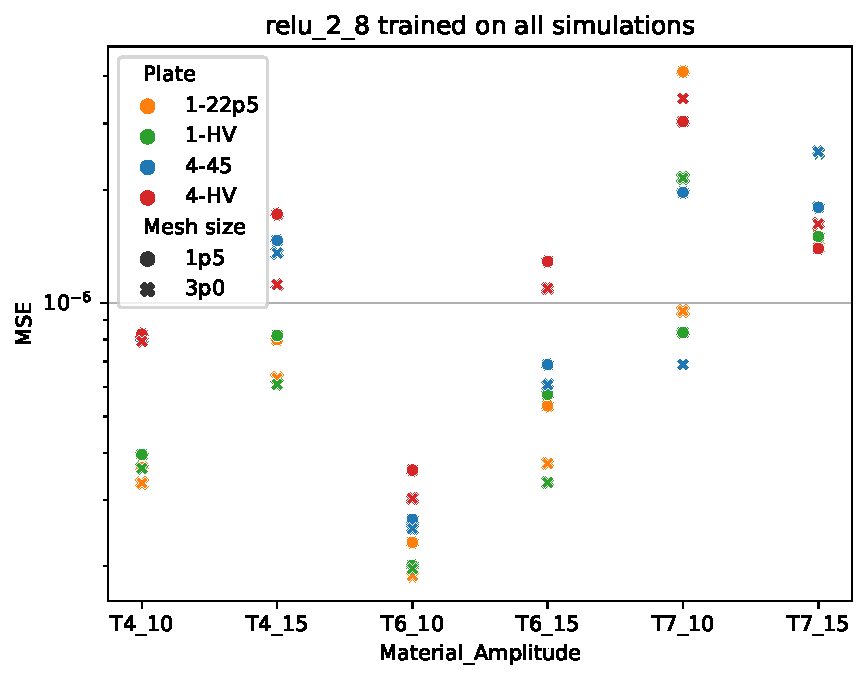
\includegraphics[width=\textwidth]{results/para4_all}
    \caption{Bottom text}
    \label{fig:para4_all}
\end{figure}

\begin{figure}
    \centering
    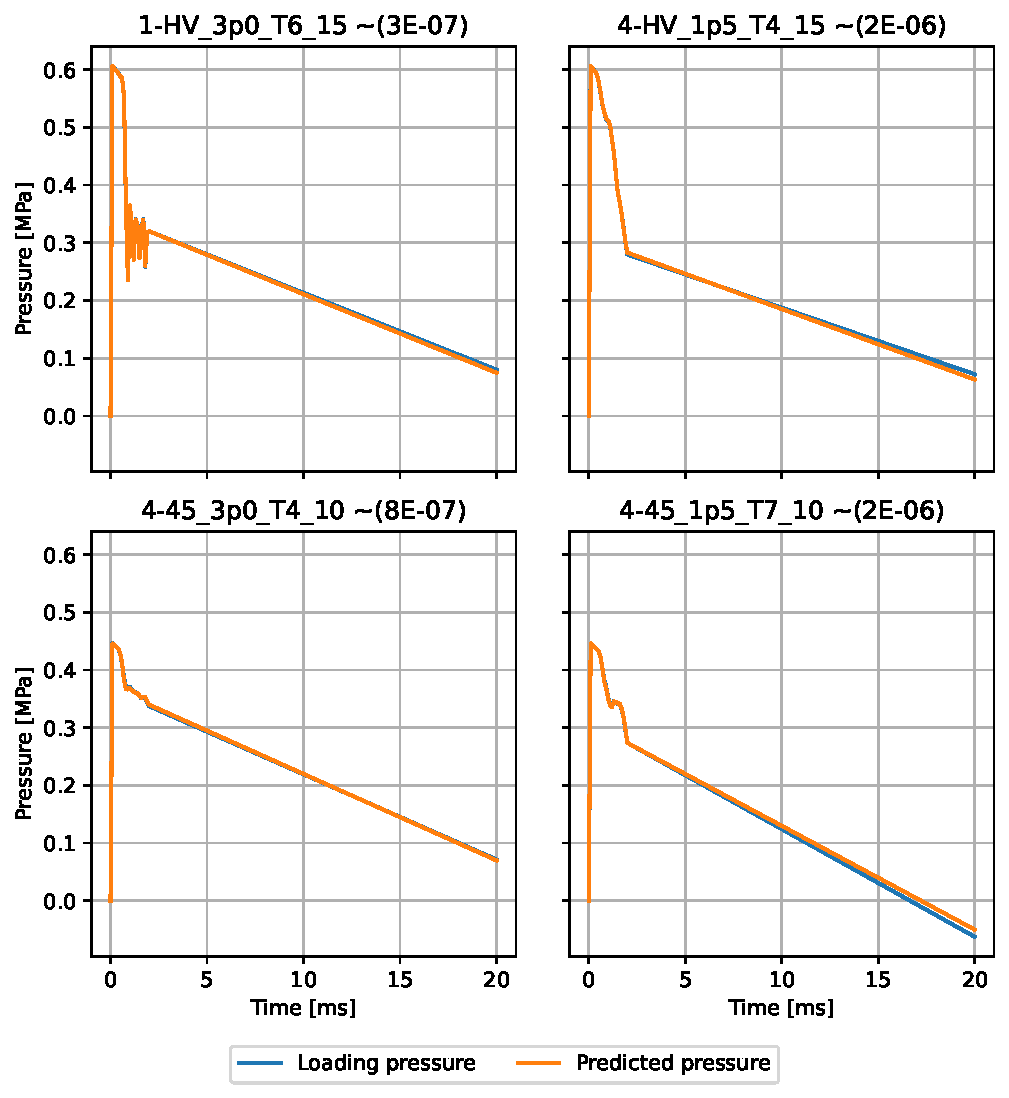
\includegraphics[width=\textwidth]{results/para4_test}
    \caption{Bottom text}
    \label{fig:para4_test}
\end{figure}

\begin{figure}
    \centering
    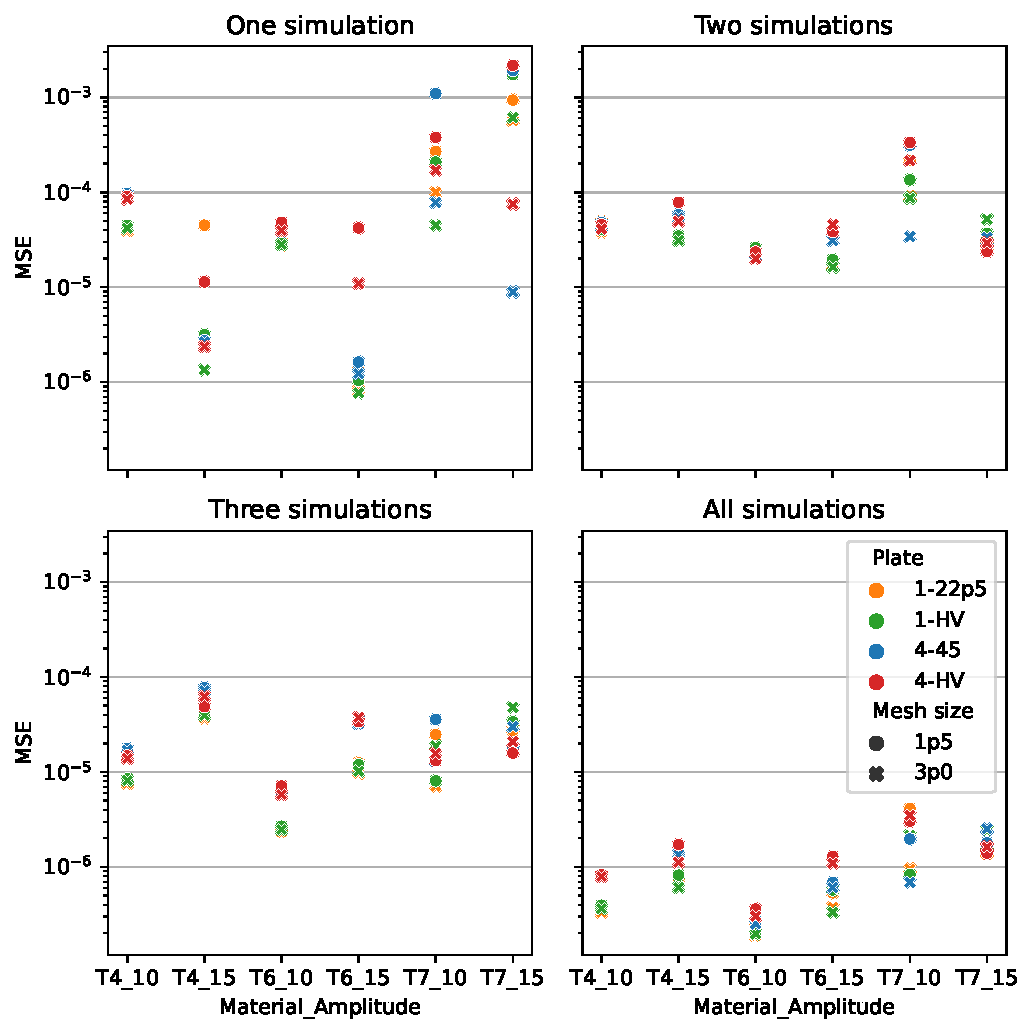
\includegraphics[width=\textwidth]{results/para_all}
    \caption{Bottom text}
    \label{fig:para_all}
\end{figure}

\begin{figure}
    \centering
    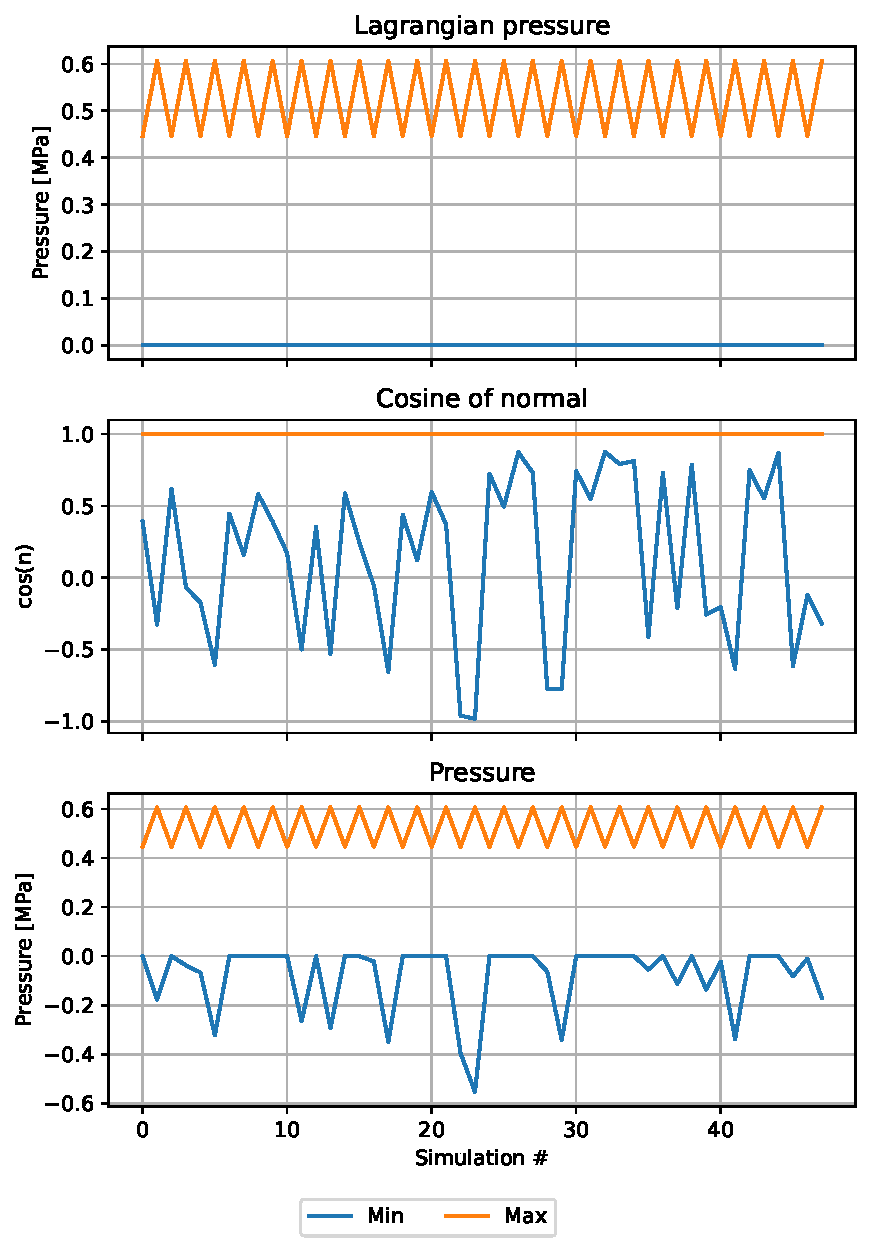
\includegraphics[width=\textwidth]{results/vars}
    \caption{Bottom text}
    \label{fig:para_vars}
\end{figure}

\begin{figure}
    \centering
    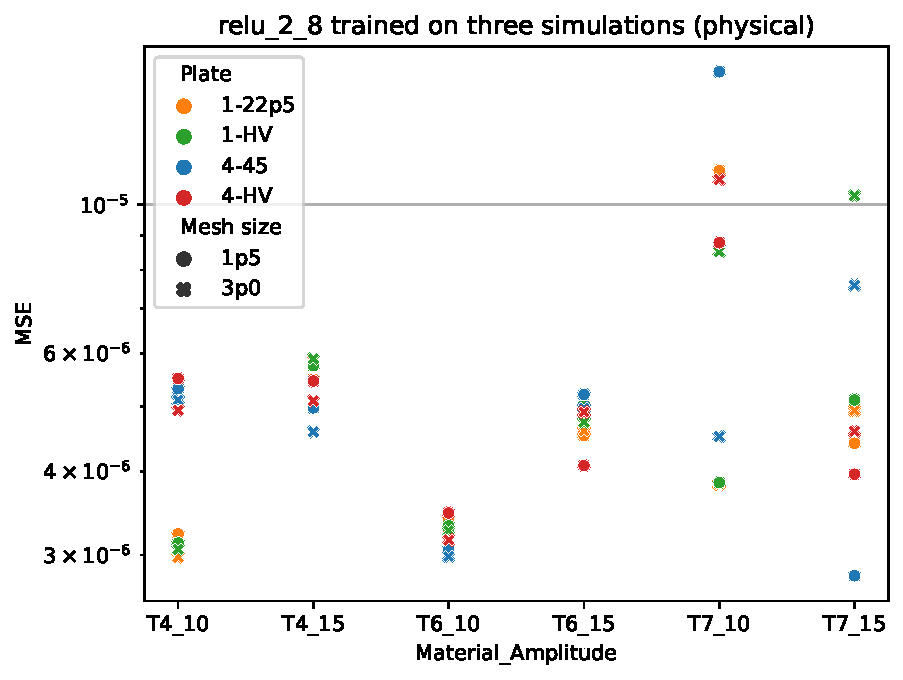
\includegraphics[width=\textwidth]{results/para5_all}
    \caption{Bottom text}
    \label{fig:para5_all}
\end{figure}

\begin{figure}
    \centering
    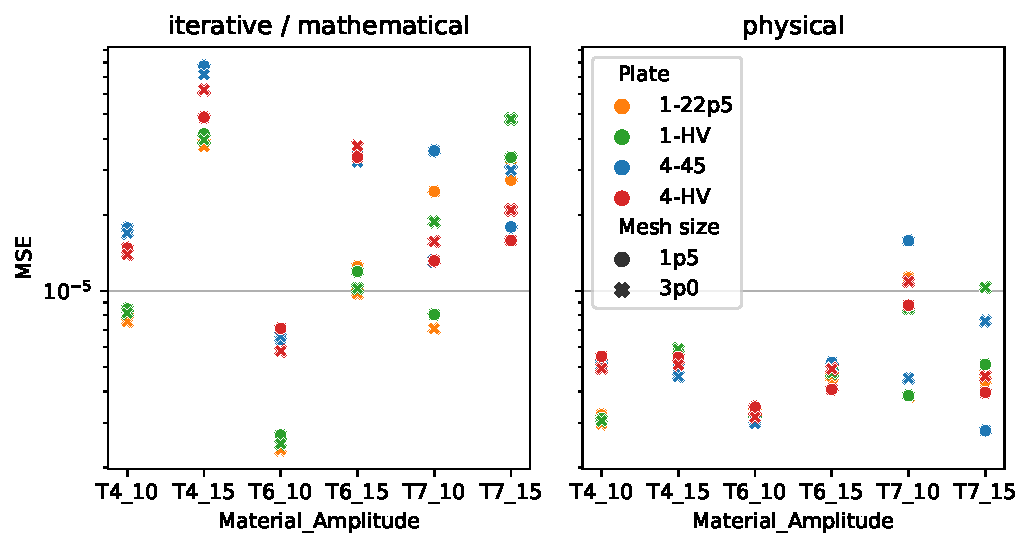
\includegraphics[width=\textwidth]{results/para3_vs_para5}
    \caption{Bottom text}
    \label{fig:para3_vs_para5}
\end{figure}

\begin{figure}
    \centering
    \begin{subfigure}[b]{0.45\textwidth}
        \centering
        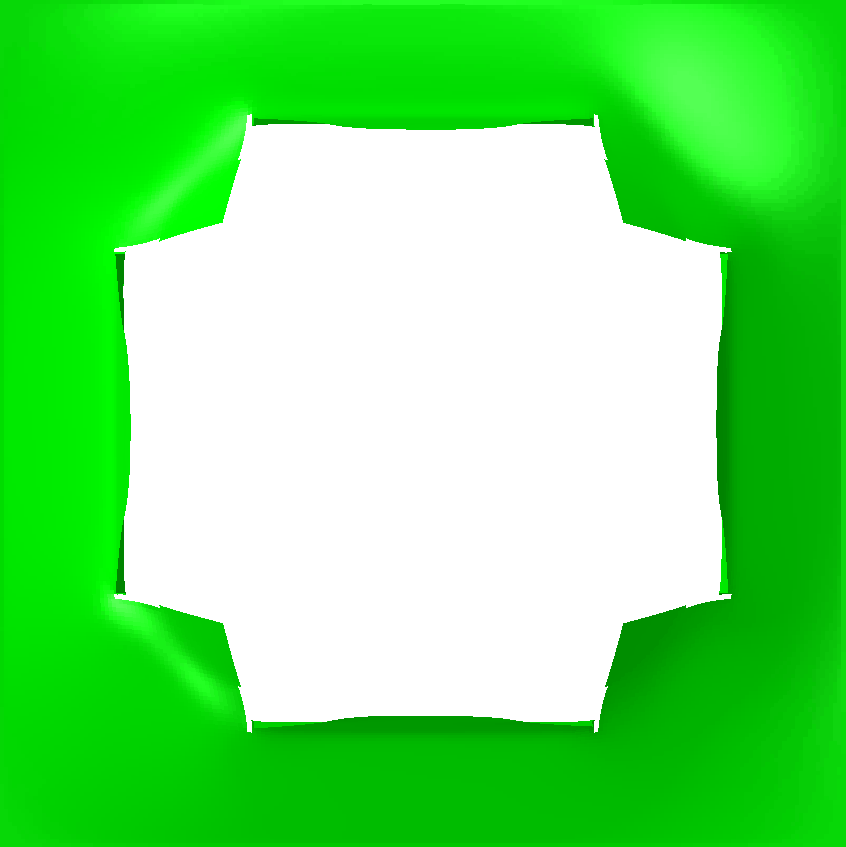
\includegraphics[width=\textwidth]{results/4-HV_1p5_T6_15}
        \caption{test}
        \label{fig:y equals x}
    \end{subfigure}
    \begin{subfigure}[b]{0.45\textwidth}
        \centering
        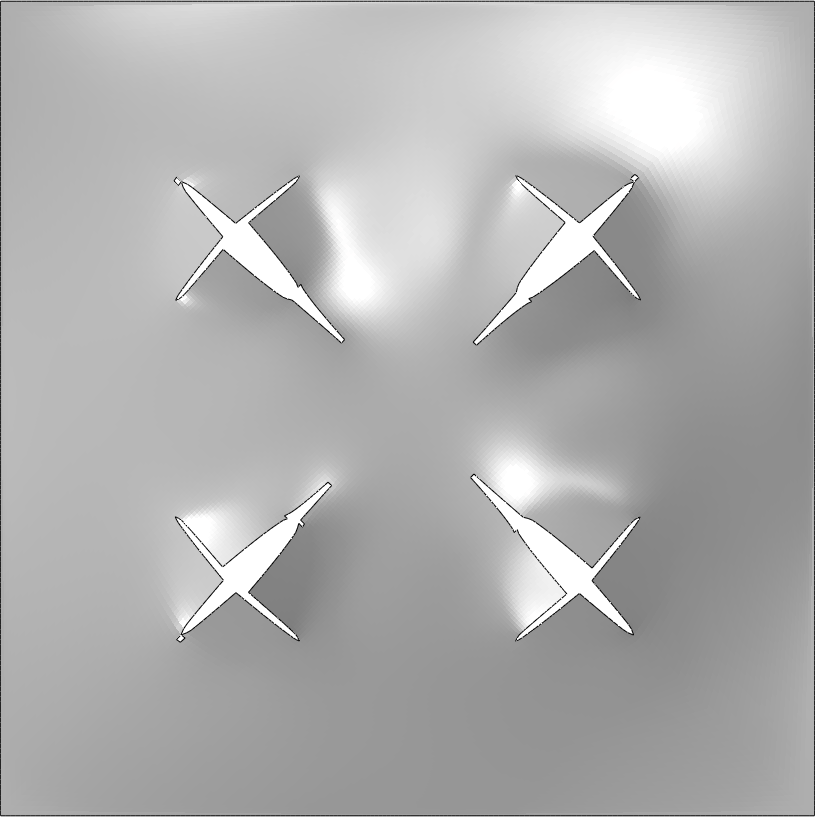
\includegraphics[width=\textwidth]{results/4-45_1p5_T6_15}
        \caption{test}
        \label{fig:three sin x}
    \end{subfigure}
    \begin{subfigure}[b]{0.45\textwidth}
        \centering
        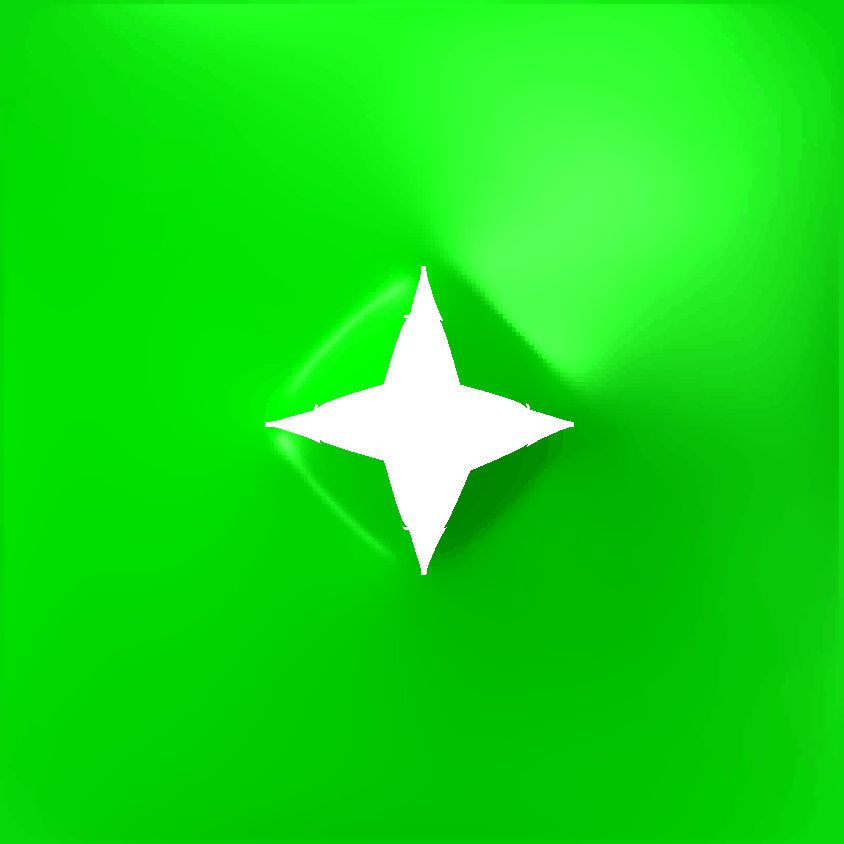
\includegraphics[width=\textwidth]{results/1-HV_1p5_T6_15}
        \caption{test}
        \label{fig:five over x}
    \end{subfigure}
    \begin{subfigure}[b]{0.45\textwidth}
        \centering
        
\includegraphics[width=\textwidth]{results/1-22p5_1p5_T6_15}
        \caption{test}
        \label{fig:blah}
    \end{subfigure}
       \caption{Effect of slits}
       \label{fig:effect_slit}
\end{figure}